\section{Framework Composition}\label{sec:physical_analysis} 
The physical layer defines the electrical and physical framework for receiving and 
transmitting signals through the media, and furthermore it defines encoding/decoding 
and alignment schemes for translating frames into signals and visa versa.

This project requires the use of DTMF tones as information carrier, and furthermore it is
required that transmission are broadcast through the air. These requirements decides some
of the properties of the physical layer, the first one is the media which is the air as 
sound waves are used for communication, and the communication can only take place as half-duplex as sending and receiving is impossible as the communication system works as a broadcast system.

\nomenclature{DTMF}{Dual-tone multi-frequency}

	\subsection{DTMF as information Carrier}
	DTMF is an abbreviation for Dual Tone Multiple Frequency. It is a system of tones that are used by
	telephones when dialing a number. The system is an arrangement of four low tones and four high tones,
	they are arranged in a four-by-four matrix which gives the system sixteen combinations.
	
	The idea is that these sixteen combinations formed by the DTMF matrix is used to transmit data
	between two or more computers. To let DTMF tones enter into data communication we have
	to apply the property of  waves to carry bits. This can be done by letting each entry in the matrix
	consist of four bits. Four bits gives sixteen combinations which each can be assigned to an entry in
	the matrix. Below is shown the DTMF map which will be used in the physical layer for encoding and decoding.
	
	\begin{table}[htb]
		\begin{center}
			\begin{tabular}{c|c c c c}
			 & 1209 Hz & 1336 Hz & 1477 Hz & 1633 Hz \\
			\hline
			697 Hz & 0000 & 0001 & 0010 & 0011 \\
			770 Hz & 0100 & 0101 & 0110 & 0111 \\
			852 Hz & 1000 & 1001 & 1010 & 1011 \\
			941 Hz & 1100 & 1101 & 1110 & 1111 \\
			\end{tabular}
		\end{center}
		\caption{Table of the matrix with the bit combinations assigned to each entry.}
		\label{tab:DTMF_mapping}
	\end{table}
	
	Now by letting one computer play the tones through a speaker and another computer record it from
	a microphone then data is transmitted. The exchange of data is essentially an exchange
	of information and it is not satisfying exchanging information of the size of four bits alone,
	cause this would make the system inefficient. The system need to be able to transmit a sequence
	of tones matching a given bit pattern. The number of tones played each second will determine the
	bit rate of the communication. As each tone hold four bits the bit rate can be written as below:
	\begin{equation}bitrate = \frac{numberOfTones \cdot numberOfBitsPerTone}{time}\end{equation}
	
	\subsection{Utilisation of PortAudio Interface}
	PortAudio exposes streams for recording or playing back sound through the sound card of a
	computer. PortAudio allow for developers to push raw audio data to the soundcards outgoing buffer and
	receiving raw audio data from the soundcards ingoing buffer. Thus, PortAudio is good foundation for the
	implementation of the physical layer as tone detecting, and tone generating algorithms can be laid on top
	of PortAudio, as basic mathematics which apply to digital signal processing. The PortAudio API provides the
	user with a callback function which implicitly exposes the sound card buffers for input and output. PortAudio
	furthermore gives the possibility for using more sound streams which then provide more callback functions
	which means that input and output streams can run asynchronously. The way PortAudio handles these streams
	will be explained in greater detail later.
	
	PortAudio will be implemented as a part of the physical layer to create the interface between the developed
	protocol stack and the sound card. An example of this is shown in figure \ref{fig:physical_4layers}.
	
	\begin{figure}[htb]
		\begin{center}
		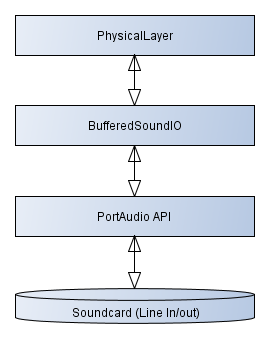
\includegraphics[scale=0.6,trim=0 0 0 0]{physical_4layers.png}%trim=l b r t
		\caption{This is a model of the steps needed to implement the physical layer. The PortAudio API is delivered
		by PortAudio. BufferedSoundIO is handling the math for generating sound and detecting sound, and also the
		PortAudio API. The physical layer includes the encoding scheme and functionality exposed to the rest of the
		developed protocol stack.}
		\label{fig:physical_4layers}
		\end{center}
	\end{figure}
	
	The DtmfPhysical and BufferedSoundIO will be implemented as two separated classes which will be bounded together
	and exposed as the physical layer to the rest of the protocol stack. The idea for implementing the physical layer
	as two seperate classes on top of PortAudio API, is to separate functionality between the physical layers internal
	layers. BufferedSoundIO class will be implementing the math needed to generate and detect tones while the physical
	layer class will implement the encoding schemes for transforming frames from the data link layer into a sequence of
	numbers which then can be pushed to BufferedSoundIO which then processes this sequence to generate a sequence of DTMF
	tones at the sending site. In the receiving site the receiving process will look a lot like the process for sending a
	frame, the BufferedSoundIO class will detect sequences of DTMF tones which will be transformed into a sequence of
	numbers. This sequence of numbers will then be sent to the DtmfPhysical and then be translated into a frame.
	
	\subsection{Goertzel Algorithm}
	To be able to detect if tones have been transmitted some algorithm for detection of tones have to be implemented.
	For this purpose the Goertzel algorithm is used, this algorithm has the ability to detect if a signal contain a
	specific frequency. Other algorithms exist which would provide the same information but those would be
	much more expensive regarding the computational complexity. Those other algorithms are called Discrete Fourier Transform (DFT)
	
	\nomenclature{DFT}{Discrete Fourier Transform}
	\nomenclature{FFT}{Fast Fourier Transform}
	
	and the other is called Fast Fourier Transform (FFT) which is a more efficient way to obtain the same information
	as the DFT algorithm. The computational complexity of DFT according to \cite[124]{DSP} is $N^2$, where N is the number of samples.
	For FFT the computational complexity is calculated to be $\frac{N}{2}\cdot \log_{2}(N)$,
	where N is the number of samples.
	
	As the detection of tones has to occur as fast as possible it is desired to lower the cost of cpu power by using 
	an algorithm which has the least computational complexity. The Goertzel algorithm therefore suit this need very well.
	The reason for this is that with a few pre-calculated constants and N iterations over N samples, a value is returned
	which indicate if a specific frequency is present in the incoming signal.
	
	Essentially the Goertzel algorithm is a second order IIR filter which is dependent on current input and previous
	output, the filter is given as the difference equation shown below:
	\begin{equation}y(n) = x(n) + 2\cdot \cos(2\pi \cdot f_{0})\cdot y(n - 1) - y(n - 2),\end{equation}
	where $f_{0}$ is the frequency of interest.
	
	By Z-transform the following is obtained:
	\begin{equation}H(z) = \frac{Y(z)}{X(z)} = \frac{1}{1 - 2\cdot \cos(2\pi \cdot f_{0})\cdot z^{-1} + z^{-2}}\end{equation}
	
	\nomenclature{IIR}{Infinite Impulse Response}
	
	As the above equation show, it is a second order IIR filter. This can be implemented as a direct form-II structure
	where the point W is of interest.
	
	\begin{figure}[htb]
		\begin{center}
		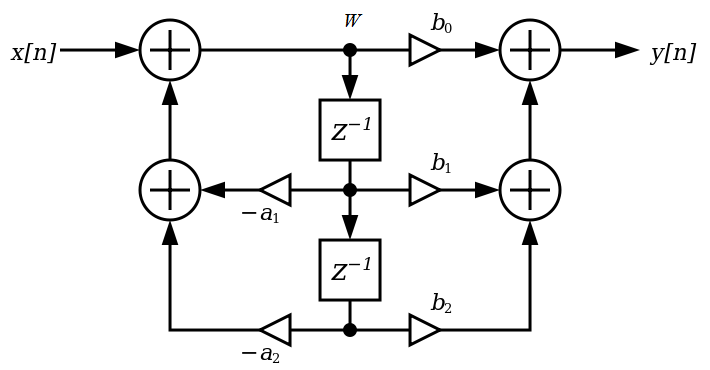
\includegraphics[scale=0.6,trim=0 0 0 0]{physical_biquad_filter.png}%trim=l b r t
		\caption{A direct form II implementation}
		\label{fig:physical_biquad_filter}
		\end{center}
	\end{figure}
	
	The point W will be used for calculating the frequency response at a specific frequency of interest. As this is taking
	place in discrete time, an expression of the frequency of interest is needed. In discrete time the frequency spectrum
	is divided into frequency bins, the size of these bins is determined by the number of samples and the sample rate.
	Obtaining the k'th bin can be done as shown below:
	\begin{equation}k = \frac{f_{0}}{f_{s}}\cdot N\end{equation}
	where $f_{0}$ is the frequency of interest, $f_{s}$ is the sampling frequency, and N is the number of samples.
	
	Now it is possible to calculate the filter coefficients, which in the case with the Goertzel algorithm reduces 
	to one single coefficient. This coefficient have to be calculated for each tone that want to be identified, but can 
	be calculated in advance because its only dependent on the frequency of interest.
	
	The coefficient is calculated with:
	\begin{equation}c = 2\cdot cos(2\pi \cdot \frac{k}{f_{s}})\end{equation}
	
	Now that all constants can be calculated in advance the detection system only have to calculate the filter output, calculate
	the magnitude of the frequency and then it is able to decide based on the result if the frequency exist in a incoming signal.
	As detection of DTMF tones is needed for this application it needs to determine if two specific frequencies is present at the
	same time. But this wont be much of a problem as the constants for each frequency can be calculated in advance.
	The algorithm are implemented as a direct form-II structure, and need to iterate over the array of collected samples to be
	able to detect if a given frequency is present in a signal.
	
	The computational complexity can therefore be written as one multiplication plus two additions per iteration per tone.
	This leads to:
	\begin{equation}numberOfOperations = 3\cdot N\cdot M,\end{equation}
	where N is the number of samples and M is the number of tones.
	
	For one tone detection over 205 samples this is around 600 calculations, for detection of 8 tones simultaneously the equation
	above result in around 5000 calculation, and these are real calculations where as for DFT and FFT the computational complexity 
	is much higher and the calculations are carried out with complex numbers.
	
	This is the reason for choosing the Goertzel algorithm for detection of frequencies.
	
	\subsection{Synchronization}
	The physical layer will be handling the synchronization of the data stream. Keeping the data in sync enables the software to
	keep track of the given chunks of data from the upper layer, this is important to do because the physical layer at the receiving
	site will have to assemble the DTMF tones back into the exact same chunks of data for delivery to the upper layer.
	A way to solve this need is to wrap the content of data into a header and possibly a tail. The chuck of data received from the 
	data link layer would be natural to wrap in a header and a tail as an extra precaution to indicate if the frame is transmitted.
	This will ease the assembly of a frame because the software have an indication of the exact start of a frame and the exact ending
	of it as well.
	
	Another problem with synchronization arise due to the mapping between 4 bit combinations and DTMF tones. This is because if there is a
	need for sending, 1111 and 1111 right after each other the system will not be able to identify the two tones corresponding to the
	given bit patterns from each other. It would therefore look like only one tone was transmitted instead of two. This actually apply
	to each combination which are followed up by its own combination of bits. Some kind of stuffing is needed to separate each tone
	from each other.
	
	There are several ways in which this problem can be solved. One of the possibilities is to stuff the transmitted tones with a little
	bit of silence in between each other. This implementation would require some sort of timing scheme which would rely on precise timing
	so decisions, on how the recorded silence should be interpreted, can be made. Decisions that will define the transmission of a frame, will be as 
	already mentioned, where does a frame start, where does it end, and the stuffing in between each tone. All these properties will be
	hard to manage duo to silence can be considered as white noise which is totally random. White noise is not in the scope of this 
	document.
	
	A second solution could be to do the stuffing at the data link layer in between equal bit patterns with a another bit pattern. 
	The are several disadvantages duo to use of this method. First the synchronization would now be spread across two layers because
	the physical layer still would have to track the beginning of a frame and the end of a frame. Another disadvantage is that this 
	method is unreliable as the defined bit pattern for stuffing at the data link layer could be generated by the data contained by the 
	frame itself. This mean that when data containing the bit pattern for stuffing this data could be discarded on false reasons and
	then corrupt the frame.
	
	A third and more elegant solution is to add a ninth frequency to the map seen in table \ref{tab:DTMF_mapping}. The new map will
	then look like the table below:
	
	\begin{table}[htb]
		\begin{center}
			\begin{tabular}{c c|c c c c}
	 		index & & 0 & 1 & 2 & 3 \\
			& DTMF & 1209 Hz & 1336 Hz & 1477 Hz & 1633 Hz \\
			\hline
			0 & 697 Hz & 0 & 1 & 2 & 3 \\
			1 & 770 Hz & 4 & 5 & 6 & 7 \\
			2 & 852 Hz & 8 & 9 & 10 & 11 \\
			3 & 941 Hz & 12 & 13 & 14 & 15 \\
			4 & 350 Hz & 16 & 17 & 18 & 19 \\
			\end{tabular}
		\end{center}
		\caption{This new mapping system create four new combinations of DTMF tones. The index notation can be used for
		implementation purpose.}
		\label{tab:newDTMF_mapping}
	\end{table}
	
	In table \ref{tab:newDTMF_mapping} a new mapping of DTMF tones is shown. This new mapping system contain four new combinations of tones
	which can be used as control signals. The combination $1209 Hz$ and $350 Hz$ gives the number 16, this number could be used as a code for
	\textit{here does the frame start}, 17 for \textit{here does the frame end}, and 18 for \textit{two equal bit patterns are presented after
	each other}. Code 19 can be leaved as a reserved control code. 
	
	\begin{table}[htb]
			\begin{center}
				\begin{tabular}{|c|c|}
				\hline
				\textbf{Code} & \textbf{Representation}\\
				\hline
				16 & Start of a frame \\
				\hline
				17 & End of a frame \\
				\hline
				18 & Double tone \\
				\hline
				19 & \textit{Reserved} \\
				\hline
				\end{tabular}
			\end{center}
			\caption{Show a table of control codes(tones).}
			\label{tab:physical_control_tones}
	\end{table}
	
	This method for synchronization is also well connected to the rest of the
	data transmission at the physical layer as the implementation is based on a tone detection system, so by adding an extra tone a lot of new
	possibilities are offered, in exchange of complicated timing schemes or sharing the synchronization functionality between two layers.
	The detection system can now by identifying a shift in tone frequencies detect a new tone was sent and thus the system is able to
	register the tone.
	
	\subsection{Encoding scheme}\label{sub:encoding_scheme}
	The encoding scheme is handling the translation from frames into DTMF tones and visa versa. The encoding will be a
	two step process as frames are translated into a sequence of numbers which then are translated into a sequence of DTMF
	tones.
	
	A frame can be considered as a stream of bits, this stream is the actual data the frame consist of. This stream can be divided
	into 4 bit sequences where each number represent the value from zero to fifteen both included. These sixteen combinations
	match up with table \ref{tab:DTMF_mapping} and the four upper rows in table \ref{tab:newDTMF_mapping}. After dividing the 
	frame into nibbles\footnote{A 4 bit size} and each nibble is put into a list, this list now is a sequence of numbers. Each
	number is assigned to a combination of two tones according to table \ref{tab:newDTMF_mapping}. These frequencies can now be
	calculated based upon the number representing each nibble.
	
	Calculate low frequency:
	\begin{equation}f_{l} = \frac{number}{4},\end{equation}
	where $f_{l}$ is a whole number, meaning if the outcome is not whole, digits after the comma are discarded. Number
	represent a number from the sequence numbers representing the data stream of a frame.
	
	Calculate high frequency:
	\begin{equation}f_{h} = number\%4,\end{equation}
	where $f_{h}$ is a whole number from the modulus operator, this operator is used here to return the rest of the division.
	
	If low and high frequencies are arranged in two arrays as they are listed, one for low tones and one for the high tones,
	then $f_{l}$ and $f_{h}$ represent an index of a tone in the frequency array concerned.
	
	The generation of numbers from identified frequencies is also an easy calculation to carry out, as this would look like this:
	\begin{equation}number = f_{l} \cdot 4 + f_{h},\end{equation}
	This can be confirmed by table \ref{tab:newDTMF_mapping}.
	
	The latter calculations defines the encoding scheme between DTMF tones and numbers, which is one of the steps needed for
	the full encoding. The other step is to get a frame and translate it into a number sequence and likewise translating a
	sequence of numbers into a frame. At the sending site frames are split into nibbles and stuffed with control tones at relevant
	spots.
	
	An Example:
	
	\begin{table}[htb]
		\begin{center}
			\begin{tabular}{|c|c|c|c|c|c|}
			\hline
			12 & 1 & 1 & 15 & 10 & 11 \\
			\hline
			\end{tabular}
		\end{center}
		\caption{Represent a frame and each number is a nibble of that frame.}
		\label{tab:physical_frame}
	\end{table}
	
	The example above would then have to be stuffed as below according to table \ref{tab:physical_control_tones}:
	
	\begin{table}[htb]
		\begin{center}
			\begin{tabular}{|c|c|c|c|c|c|c|c|c|}
			\hline
			16 & 12 & 1 & 18 & 1 & 15 & 10 & 11 & 17 \\
			\hline
			\end{tabular}
		\end{center}
		\caption{Represent a frame as the number sequence after stuffing it.}
		\label{tab:physical_stuffed_frame}
	\end{table}
	
	As seen in table \ref{tab:physical_stuffed_frame} the frame itself is wrapped in control codes telling the software where
	the frame start and end. In between nibbles of the same bit combination a control code is added to indicate that two equal
	tones are going to be played right after another as this frame is transmitted.
